\section{Dart}
\label{dart}

\subsection{Was ist Dart?}

\textit{Dart} ist eine höhere, clientoptimierte Programmiersprache zur Entwicklung von Apps auf mehreren Plattformen.

Sie wird von \textit{Google} entwickelt und wird hauptsächlich zum Entwickeln von Serversoftware, (nativen) Mobile-, Desktop- oder Web-Apps verwendet.

Wie viele andere Hochsprachen baut Dart strikt auf dem Konzept der Objekt-Orientierung auf und ist eine klassenbasierte Programmiersprache mit eingebautem, automatischem
Garbage-Collector.

Dart ist eine kompilierte Sprache und kann sowohl in Maschinencode als auch in Vanilla-JavaScript kompiliert werden, wodurch plattformunabhängige Entwicklung ermöglicht 
wird.

\subsection{Syntax von Dart}

Die Syntax von Dart sieht auf den ersten Blick aus, wie eine Mischung aus \textit{Java} und \text{JavaScript}.

Ein \textit{Hello-World}-Programm würde in Dart also folgendermaßen aussehen:

\begin{code}[h]
    \centering
    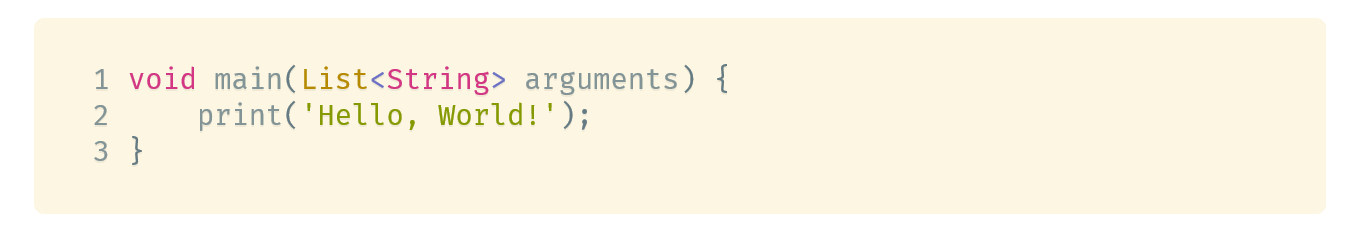
\includegraphics[width=1\textwidth]{images/Dart/theory/dartHelloWorld.png}
    \vspace{-25pt}
    \caption{Einfaches Hello-World-Programm in Dart}
\end{code}

\subsubsection{Variablen}

Die Deklaration von Variablen funktioniert gleich wie in anderen Hochsprachen, so werden Primitiv- und Referenzdatentypen gleich wie in Java deklariert (int, char, byte bzw. Integer, String, Boolean ...).

Alternativ kann auf das Schlüsselwort \textit{var} aus JavaScript zurückgegriffen werden. Dieses ist vergleichbar mit dem \textit{Object}-Datentyp aus Java und \glqq errät\grqq\space den benötigten Typ der entsprechenden Variable.

\begin{code}[h]
    \centering
    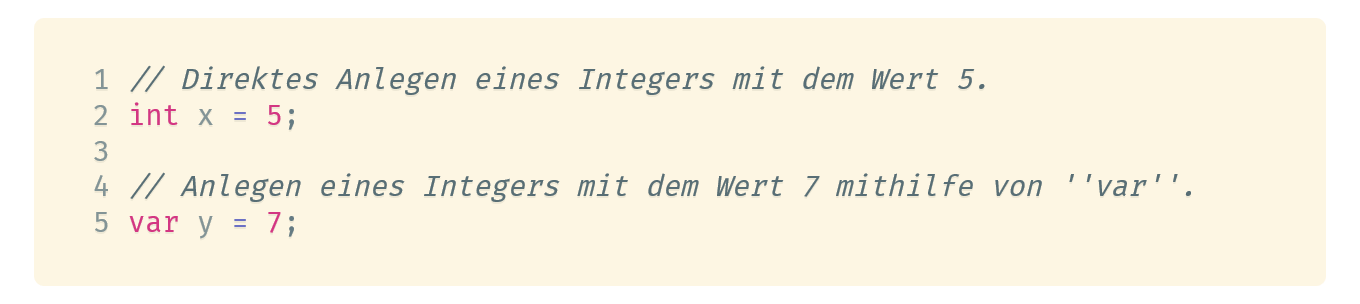
\includegraphics[width=1\textwidth]{images/Dart/theory/dartVariables.png}
    \vspace{-25pt}
    \caption{Anlegen einfacher Variablen in Dart}
\end{code}

Nach Dart-Konventionen ist es allerdings üblich, die Angabe des Datentyps für Variablen im lokalen Scope, beispielsweise innerhalb einer Funktion, durch das \textit{var}-Keyword zu ersetzen. \cite{dartdesignvariables2021}

Für \textit{finale} Variablen kann sowohl auf dezidierte Datentypen als auch auf \textit{var} verzichtet werden, bei der Deklaration von Referenzdatentypen kann das \textit{new}-Keyword 
weggelassen werden.

\begin{code}[h]
    \centering
    \includegraphics[width=1\textwidth]{images/Dart/theory/dartLocalFinal.png}
    \vspace{-25pt}
    \caption{Finale Variable im lokalen Scope}
\end{code}

\subsubsection{Verzweigungen und Schleifen}

Für die Kontrolle des Ablaufs eines Programms werden wie gewohnt \textit{if-else-Statements} und Schleifen
wie \textit{for / for in / for each} oder \textit{while} verwendet.

Die Syntax jener Kontrollstrukturen ist mit der von JavaScript quasi ident.

\begin{code}[h]
    \centering
    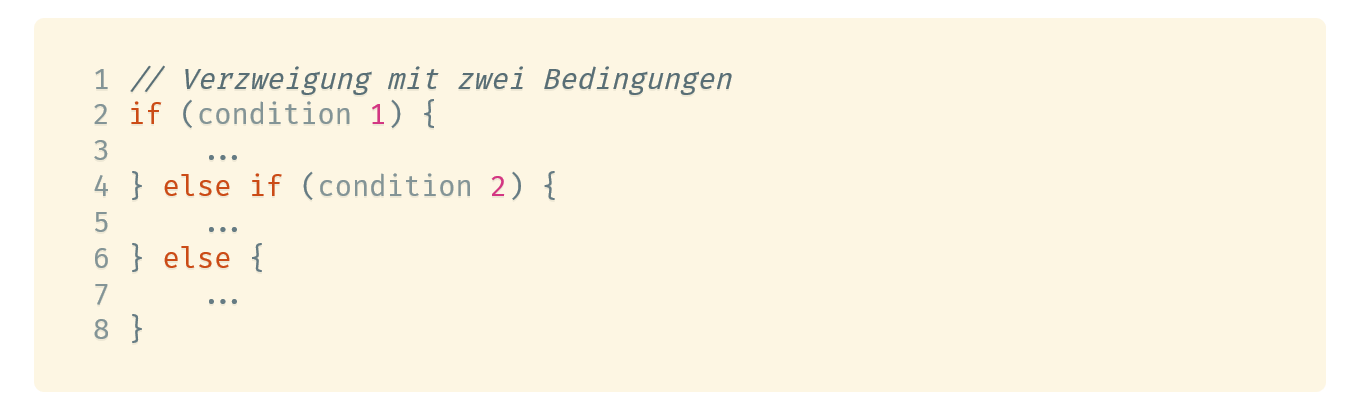
\includegraphics[width=1\textwidth]{images/Dart/theory/dartConditional.png}
    \vspace{-25pt}
    \caption{Conditional mit zwei Bedingungen}
\end{code}

\begin{code}[h]
    \centering
    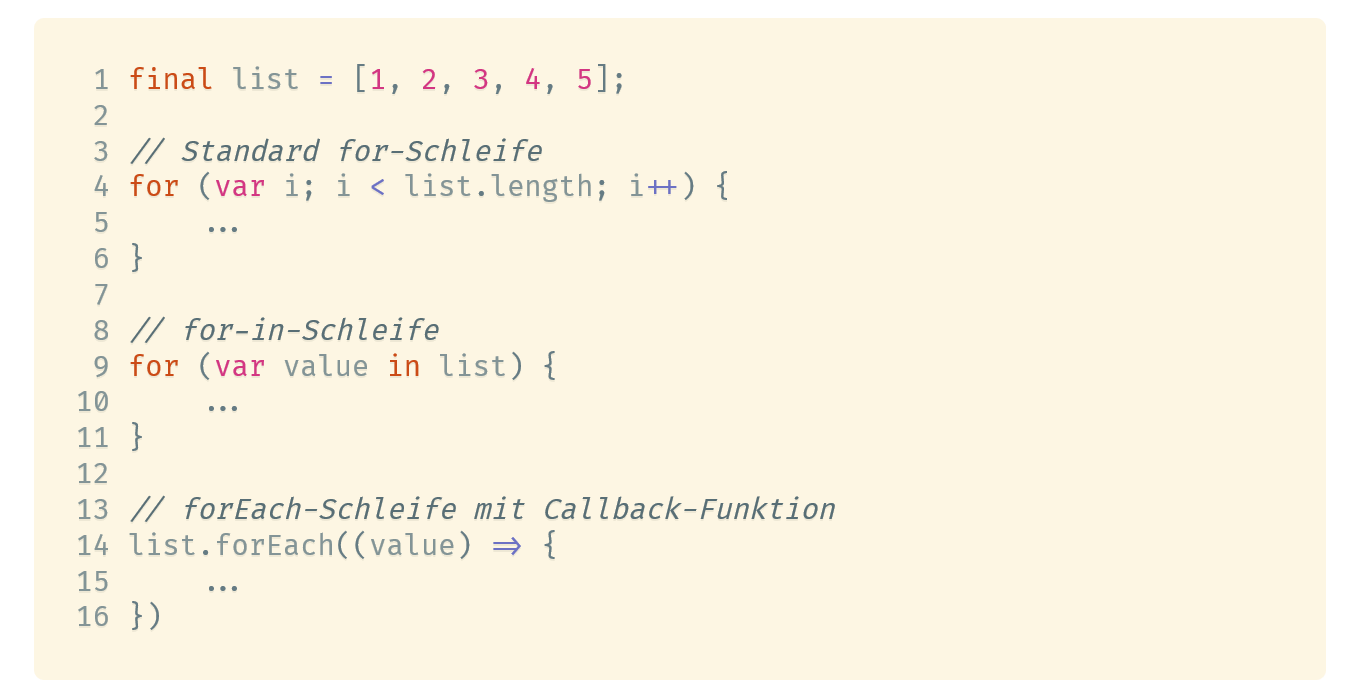
\includegraphics[width=1\textwidth]{images/Dart/theory/dartForLoop.png}
    \vspace{-25pt}
    \caption{Arten von for-Schleifen in Dart}
\end{code}

\begin{code}[h]
    \centering
    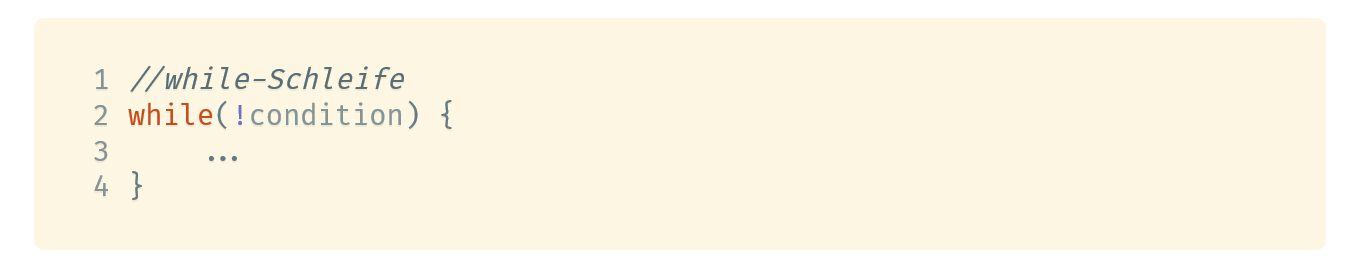
\includegraphics[width=1\textwidth]{images/Dart/theory/dartWhileLoops.png}
    \vspace{-25pt}
    \caption{While-Schleife in Dart}
\end{code}

\newpage

\subsubsection{Funktionen}

Funktionen in Dart werden auf dieselbe Weise wie in Java deklariert. Die Funktionssignatur bzw. der Funktionskopf benötigt den Rückgabewert der Funktion, den Namen und die Parameterliste.

\begin{code}[h]
    \centering
    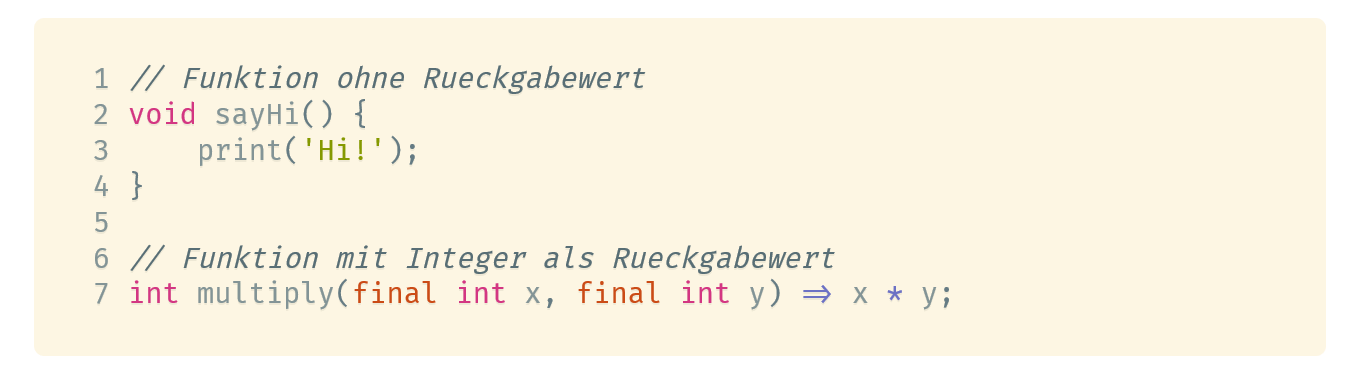
\includegraphics[width=1\textwidth]{images/Dart/theory/dartFunctions.png}
    \vspace{-25pt}
    \caption{Deklarieren von Funktionen in Dart}
\end{code}

\newpage

Dart bietet in Bezug auf das Übergeben von Parametern an eine Funktion mehrere Mögichkeiten:

\begin{itemize}
    \item \textit{positioned, optional parameters}
    \item \textit{named, optional parameters}
\end{itemize}

Sogenannte \textit{positionierte und optionale Parameter} werden in der Argumentliste einer Funktion mithilfe eckiger Klammern gekennzeichnet und bewirken, wie der Name bereits verrät, dass jene Parameter optional und in ihrer Position fixiert sind.

\begin{code}
    \centering
    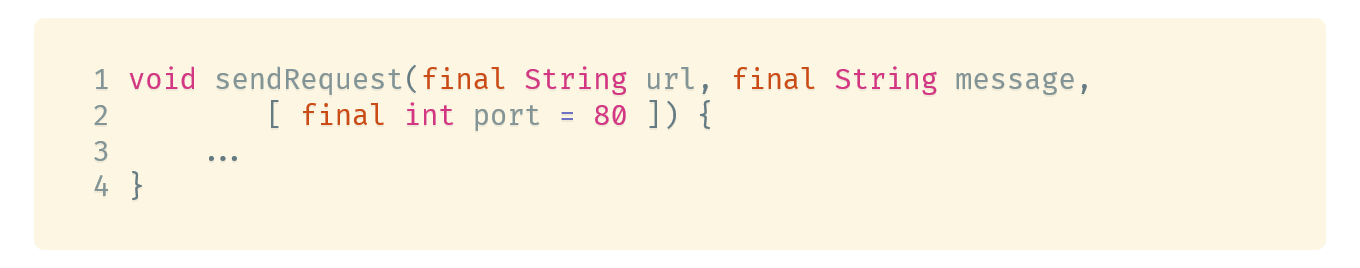
\includegraphics[width=1\textwidth]{images/Dart/theory/dartPositionedArgumentsFunction.png}
    \vspace{-25pt}
    \caption{Funktion mit positioned, optional Parametern}
\end{code}

Die Funktion \textit{getHttpUrl()} benötigt neben dem Server und Pfad auch eine Portnummer, welche hier als positionierter, optionaler Parameter mit einem Standartwert von 80 festgelegt wird.

Wird beim Aufruf dieser Funktion der Port-Integer weggelassen, so wird dieser immer auf 80 gesetzt.

\begin{code}
    \centering
    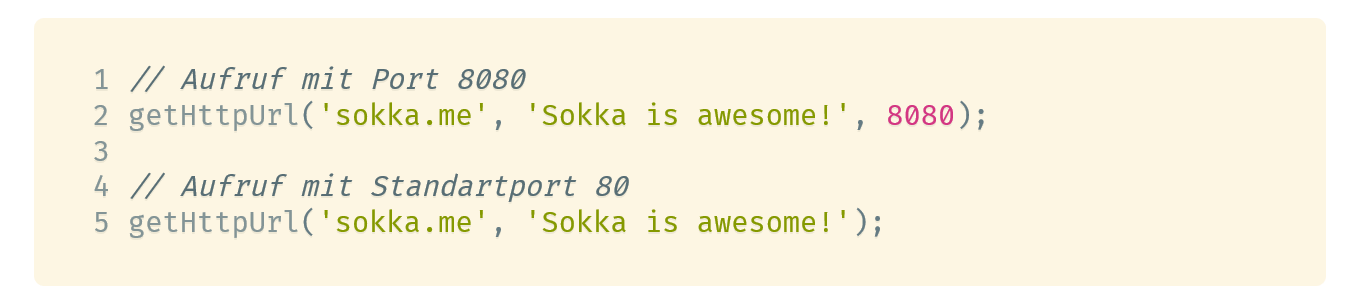
\includegraphics[width=1\textwidth]{images/Dart/theory/dartCallPositionedFunction.png}
    \vspace{-25pt}
    \caption{Aufrufen einer Funktion mit positioned Parametern}
\end{code}

\newpage

Neben positionierten Parametern gibt es noch \glqq benannte\grqq , sogenannte \textit{named} Parameter, die mit geschwungenen Klammern in der Parameterliste deklariert werden.

\begin{code}
    \centering
    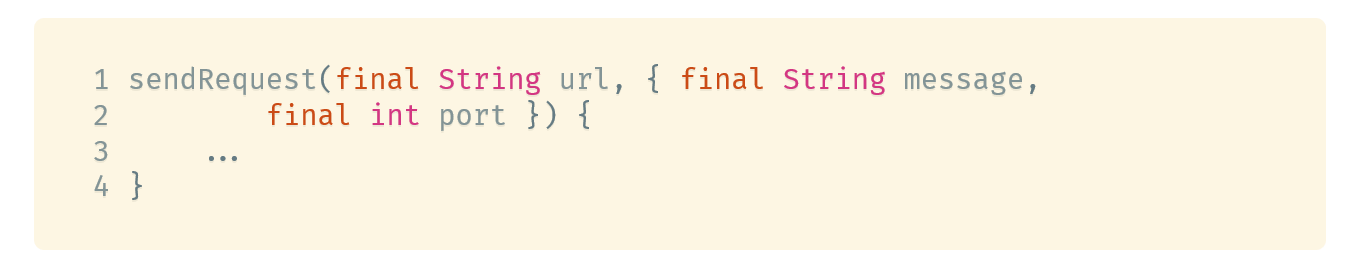
\includegraphics[width=1\textwidth]{images/Dart/theory/dartNamedArguments.png}
    \vspace{-25pt}
    \caption{Aufrufen einer Funktion mit named Parametern}
\end{code}

Neben einer URL benötigt die obige Funktion auch eine Nachricht und eine Port-Nummer, um einen gültigen Request zu versenden. Aufgrund ihrer Deklaration innerhalb der geschwungenen Klammern
werden sie als benannte Parameter interpretiert und werden wie folgt übergeben.

\begin{code}[h]
    \centering
    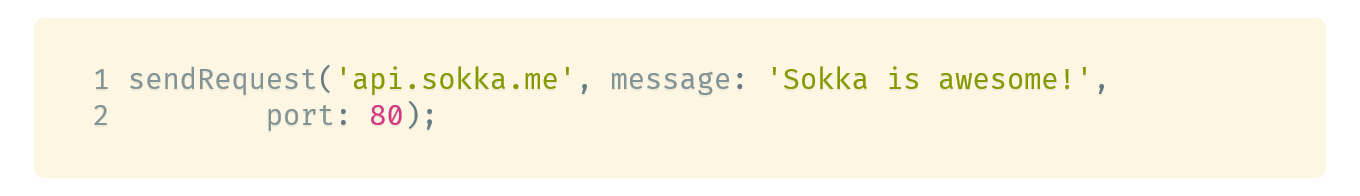
\includegraphics[width=1\textwidth]{images/Dart/theory/dartCallNamedArguments.png}
    \vspace{-25pt}
    \caption{Aufrufen einer Funktion mit \textit{named} Parametern}
\end{code}

\begin{code}[h]
    \centering
    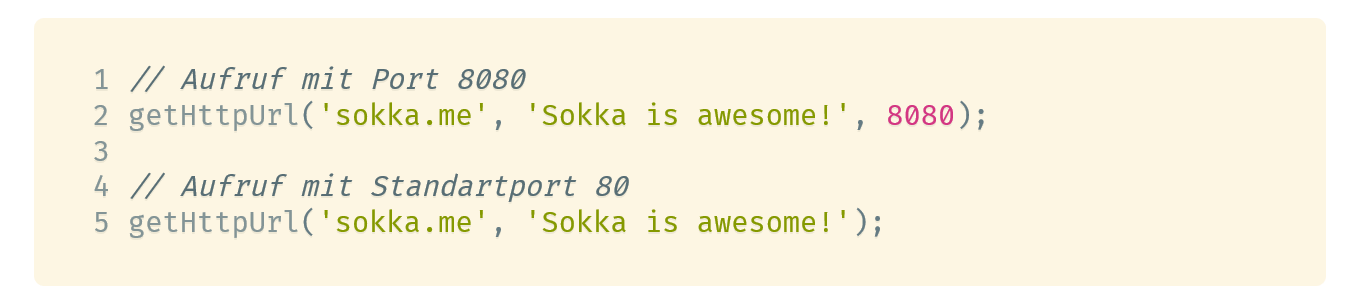
\includegraphics[width=1\textwidth]{images/Dart/theory/dartCallPositionedFunction.png}
    \vspace{-25pt}
    \caption{Aufrufen einer Funktion mit \textit{positioned} Parametern}
\end{code}

\newpage

\subsubsection{Klassen}

Ähnlich zu Hochsprachen wie Java oder C\# können auch in Dart einfach Klassen erstellt werden, wie nachfolgend zu sehen ist.

\begin{code}[h]
    \centering
    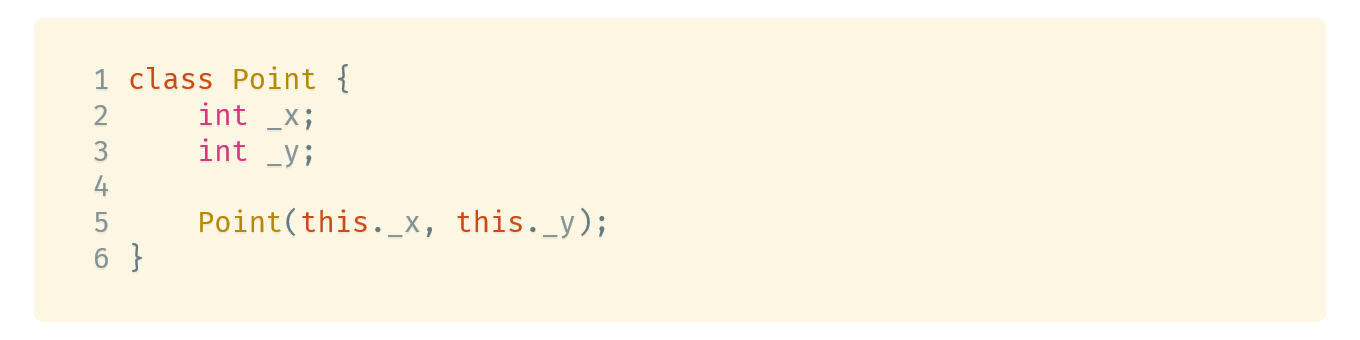
\includegraphics[width=1\textwidth]{images/Dart/theory/dartClass.png}
    \vspace{-25pt}
    \caption{Simple Klassen in Dart}
\end{code}

Wie auch in JavaScript oder Python gibt es in Dart keine Access-Modifier, um den Zugriff auf Felder, Methoden oder Klassen zu regulieren. Felder und Funktionen sind standardmäßig \textbf{public} und können lediglich durch einen Unterstrich zu Beginn des Feld- bzw. Funktionsnamen als \textbf{private} gekennzeichnet werden.

Desweiteren stehen in Dart, ebenso wie in C\#, die Schlüsselwörter \textbf{get} und \textbf{set} zur Verfügung, mit deren Verwendung Funktionen als dezidierte Getter- bzw.
Setter-Funktion für eine Membervariable definiert werden können.

\begin{code}[h]
    \centering
    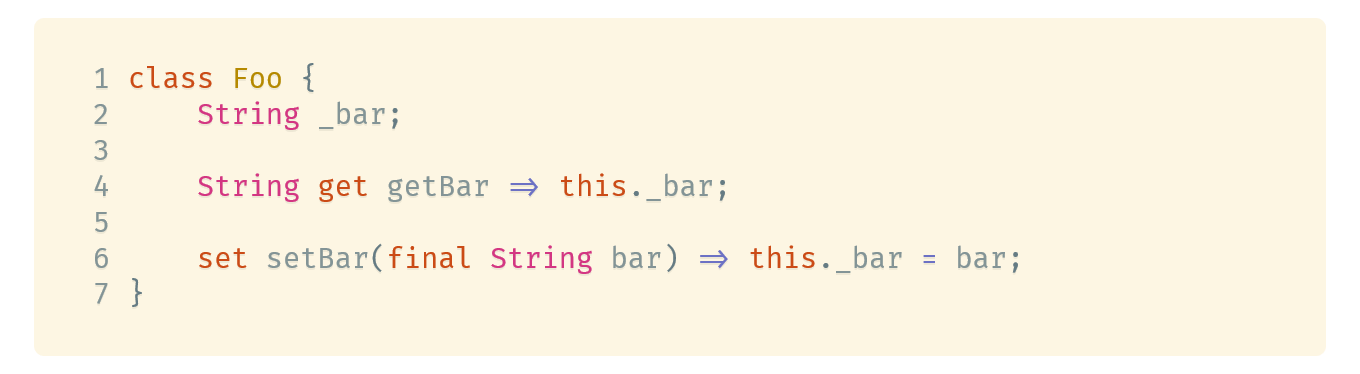
\includegraphics[width=1\textwidth]{images/Dart/theory/dartGetterSetter.png}
    \vspace{-25pt}
    \caption{Getter- und Setter-Funktionen in Dart}
\end{code}

In diesem Beispiel werden \textit{getBar} und \textit{setBar} als dezidierte Getter- und Setter-Funktion für das Feld \textbf{\_bar} festgelegt. Auffällig ist ebenso die JavaScript-ähnliche Arrow-Syntax, die ein Return-Statement zur Gänze ersetzen kann.

So kann ein \textit{return}, wie es in Java geschrieben wird, durch ein Arrow-Statement wie folgt
ersetzt werden.

\begin{code}[h]
    \centering
    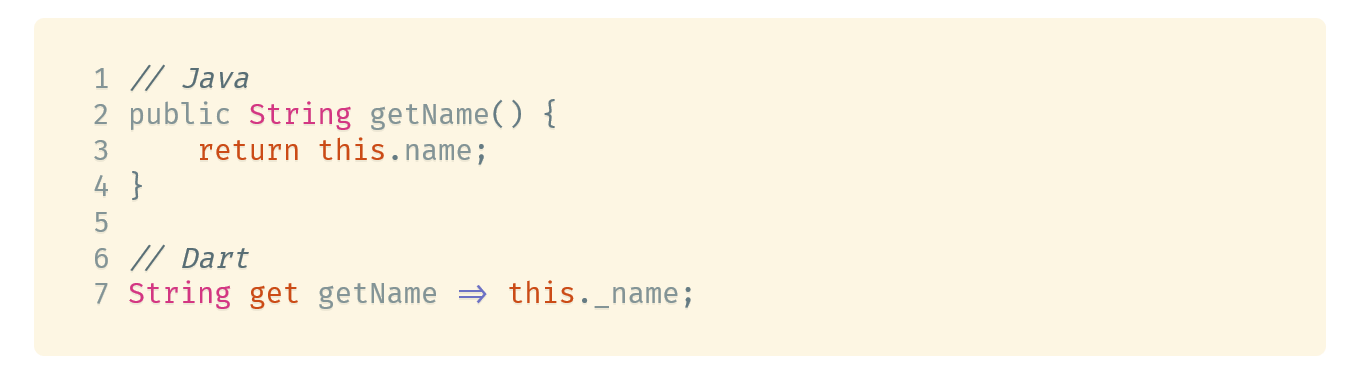
\includegraphics[width=1\textwidth]{images/Dart/theory/dartVSJavaGetter.png}
    \vspace{-25pt}
    \caption{Vergleich einer Getter-Funktion zwischen Java und Dart}
\end{code}

\newpage

\subsubsection{Vererbungsstrukturen}

\paragraph{Abstrakte Klassen}

% https://dart.dev/guides/language/language-tour#abstract-classes

Um eine Klasse als abstrakt zu definieren wird in Dart das \textit{abstract}-Keyword verwendet und mittels
\textit{extends}-Keyword an andere Klassen vererbt.

\begin{code}[h]
    \centering
    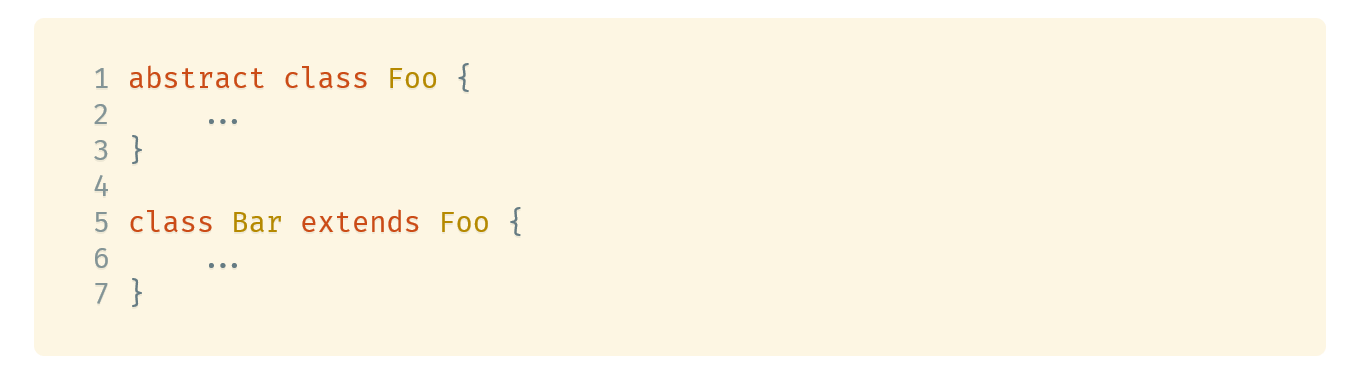
\includegraphics[width=1\textwidth]{images/Dart/theory/dartAbstractClass.png}
    \vspace{-25pt}
    \caption{Erzeugen und Vererben abstrakter Klassen in Dart}
\end{code}

\paragraph{Interfaces}
 
% https://dart.dev/guides/language/language-tour#implicit-interfaces

Dart unterstützt das Prinzip von sogenannten \textit{impliziten Interfaces}. Das heißt, dass jede erzeugte Klasse automatisch als ein Interface genutzt und implementiert werden kann.
